\documentclass[border=3pt]{standalone}
\usepackage{tikz}
\usetikzlibrary{arrows.meta,calc,positioning}
\tikzset{pin/.style={-{Stealth[length=5pt]}, thick},
  blk/.style={draw, thick, font=\sffamily\small, align=center}}
\begin{document}
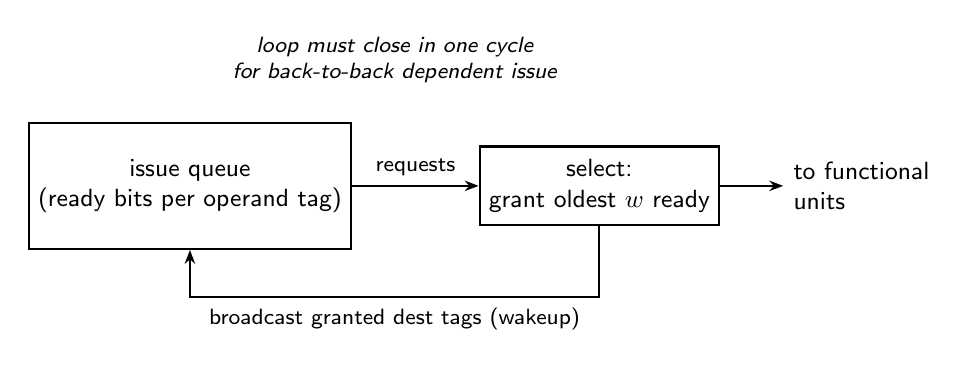
\begin{tikzpicture}[font=\sffamily\small]
  \node[blk, minimum width=34mm, minimum height=16mm] (iq) at (0,0) {issue queue\\(ready bits per operand tag)};
  \node[blk, minimum width=22mm, minimum height=10mm] (sel) at (5.2,0) {select:\\grant oldest $w$ ready};
  \draw[pin] (iq.east) -- node[above, font=\sffamily\footnotesize]{requests} (sel.west);
  \draw[pin] (sel.south) |- node[below, pos=0.75, font=\sffamily\footnotesize]{broadcast granted dest tags (wakeup)} ($(iq.south)+(0,-6mm)$) -| (iq.south);
  \draw[pin] (sel.east) -- ++(8mm,0) node[right, align=left, font=\sffamily\small]{to functional\\units};
  \node[font=\sffamily\footnotesize\itshape, align=center] at (2.6,1.6) {loop must close in one cycle\\for back-to-back dependent issue};
\end{tikzpicture}
\end{document}
